% Time-memory-data cryptanalysis of the HiTag2 stream cipher
%
% Presentation file
% Rajesh Bachani

\documentclass{beamer}
\setbeamertemplate{navigation symbols}{}

\usepackage[english]{babel}
\usepackage[latin1]{inputenc}
\usepackage{graphicx}
\usepackage{colortbl}
\usepackage{url}
\usepackage{beamerthemeshadow}
\usepackage[english]{babel}
% or whatever

\usepackage[latin1]{inputenc}
% or whatever

\mode<presentation>
{
  \usetheme{Warsaw}
  % or ...

  \setbeamercovered{transparent}
  % or whatever (possibly just delete it)
}

% Delete this, if you do not want the table of contents to pop up at
% the beginning of each subsection:
\AtBeginSubsection[]
{
  \begin{frame}<beamer>{Outline}
    \tableofcontents[currentsection,currentsubsection]
  \end{frame}
}

% If you wish to uncover everything in a step-wise fashion, uncomment
% the following command: 

%\beamerdefaultoverlayspecification{<+->}


% the document begins here

\begin{document}
\title{Time-memory-data cryptanalysis of the HiTag2 stream cipher}
\subtitle{M.Sc. project presentation}

\author{Rajesh Bachani}

\institute
{
  Department of Mathematics\\
  Technical University of Denmark
}

\date
{
	Supervisor: Dr.~Erik Zenner
}

\begin{frame}
  \titlepage
\end{frame}

\begin{frame}{Outline}
  \tableofcontents
\end{frame}

\section{Introduction}

\subsection{Basics}

\begin{frame}{Cryptography}

  \begin{itemize}
  \item Cryptography provides data confidentiality, integrity, authentication, non-repudiation etc. 
  \item Main ideas: encryption, decryption and `secret key'
  \item Cryptosystems can be symmetric-key or asymmetric-key
  \item Symmetric-key cryptosystems are further divided into two categories: 
  	\begin{itemize}
  		\item Block cipher
  		\item Stream cipher
  	\end{itemize}
  \end{itemize}
\end{frame}

\begin{frame}{One-time pad}
  \begin{itemize}
  \item OTP provides the basic design principle for stream ciphers
  \item A random key is chosen and \textit{xor}'ed with plaintext, bitwise
  \end{itemize}
  
  \begin{figure}[htp]
	\centering
	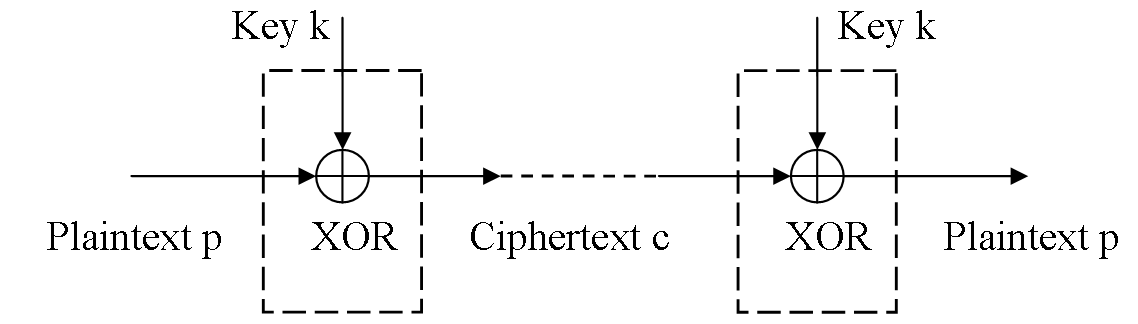
\includegraphics[width = 3in]{./figures/one-time-pad.PNG}
	\end{figure}
	
	\begin{itemize}
		\item OTP exhibit perfect secrecy, but suffer from the following problems:
  	\begin{enumerate}
  		\item Long and random key is required
  		\item Key can be used just once
  	\end{enumerate}
  \end{itemize}
\end{frame}


\begin{frame}{Pseudo-random number generator}
	
	
	\begin{itemize}
		\item PRSG generates a long pseudo-random \textit{keystream} using a short key
		\item The same key can be re-used by using a different initialization parameter for every run of the cipher
	\end{itemize}
	
  \begin{figure}[htp]
	\centering
	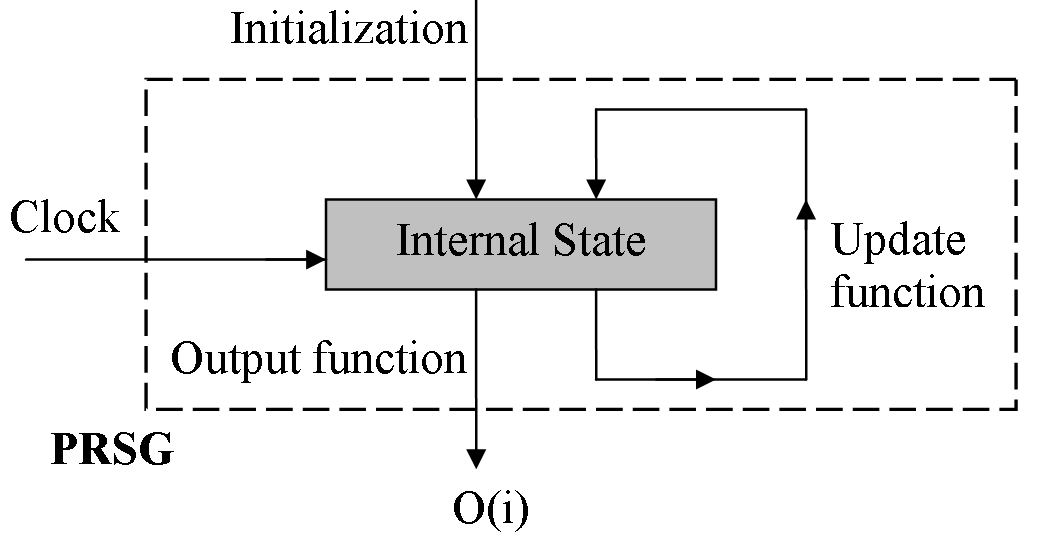
\includegraphics[width = 2.5in]{./figures/prsg.PNG}
	\end{figure}

\end{frame}

\begin{frame}{Internal model of stream cipher}

  \begin{figure}[htp]
	\centering
	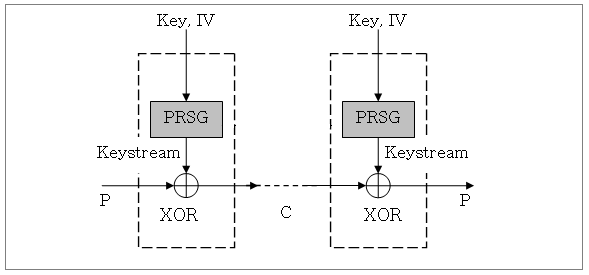
\includegraphics[width = 2.5in]{./figures/stream-cipher.PNG}
	\end{figure}

	\begin{itemize}
		\item The perfect secrecy of OTP does not apply here as the keystream is pseudo-random in nature
	\end{itemize}
\end{frame}

\begin{frame}{Linear feedback shift register}
	\begin{itemize}
		\item Linear feedback shift register (LFSR) is one way to implement PRSG

	\end{itemize}
	\begin{columns}
	
	\begin{column}{5cm}
	\begin{figure}[htp]
	\centering
	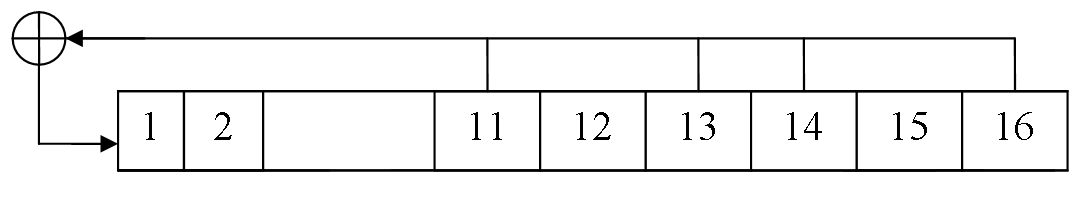
\includegraphics[width = 2in]{./figures/lfsr-example.PNG}
	\end{figure}
	\end{column}
	
	\begin{column}{5cm}
	\begin{figure}[htp]
	\centering
	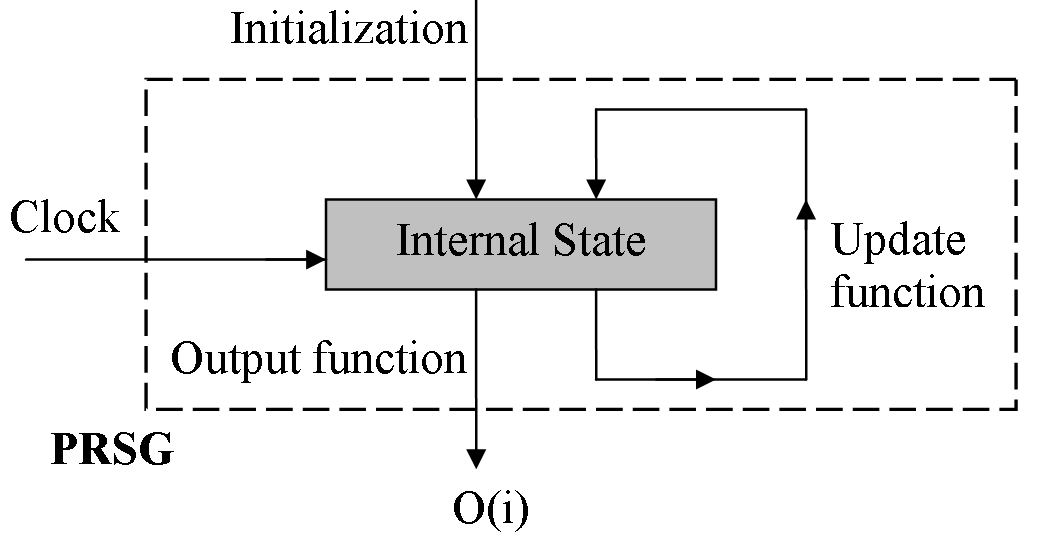
\includegraphics[width = 2in]{./figures/prsg.PNG}
	\end{figure}
	\end{column}	

	\end{columns}
\end{frame}	
	



%\begin{frame}{Make Titles Informative}
%
%  You can create overlays\dots
%  \begin{itemize}
%  \item using the \texttt{pause} command:
%    \begin{itemize}
%    \item
%      First item.
%      \pause
%    \item    
%      Second item.
%    \end{itemize}
%  \item
%    using overlay specifications:
%    \begin{itemize}
%    \item<3->
%      First item.
%    \item<4->
%      Second item.
%    \end{itemize}
%  \item
%    using the general \texttt{uncover} command:
%    \begin{itemize}
%      \uncover<5->{\item
%        First item.}
%      \uncover<6->{\item
%        Second item.}
%    \end{itemize}
%  \end{itemize}
%\end{frame}

\subsection{Time-memory tradeoff attacks}

\begin{frame}{Brute force attack}
\end{frame}

\begin{frame}{Precomputed ciphertext attack}
\end{frame}

\begin{frame}{Tradeoff attack}
\end{frame}

\begin{frame}{Birthday paradox}
\end{frame}

\subsection{HiTag2 stream cipher}

\begin{frame}{Background}
\begin{itemize}
\item HiTag2 stream cipher is used for remote keyless entry in cars by providing two-way authentication between car and car key
\item It was a proprietary algorithm of Philips Semiconductors (now NXP)
\item HiTag2 was reverse-engineered from its software implementation recently
\end{itemize}
\end{frame}

\begin{frame}{Design}
\begin{itemize}
	\item Components of HiTag2:
	\begin{itemize}
		\item 48 bit key
		\item 32 bit serial ID
		\item 32 bit initialization vector (IV)
		\item 48 bit internal state with linear update function (basically, an LFSR)
		\item Non-linear output function based on multiplexor
	\end{itemize}
	
	\item Cipher is initialized in the following three phases:
	\begin{itemize}
		\item LFSR initialization
		\item LFSR setup
		\item Keystream generation
	\end{itemize}

\end{itemize}
\end{frame}

\begin{frame}{LFSR initialization and setup}
\begin{itemize}
	\item \small{Internal state is initialized using the serial ID and least significant 16 bits of secret key}
\end{itemize}
	\begin{figure}[htp]
	\centering
	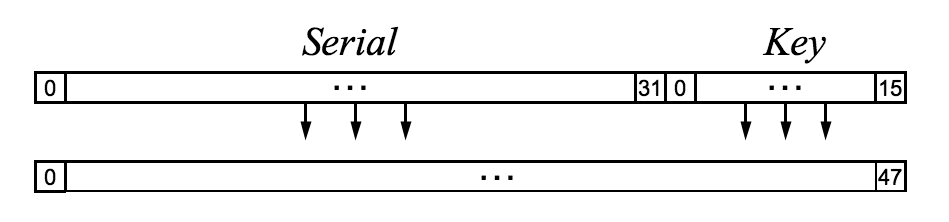
\includegraphics[width = 2.1in]{./figures/hitag2-1.PNG}
	\end{figure}
\begin{itemize}
		\item \small{During setup, one bit each from the key, the IV and the output are \textit{xor}'ed and result is used as new bit for the internal state}
\end{itemize}

	\begin{figure}[htp]
	\centering
	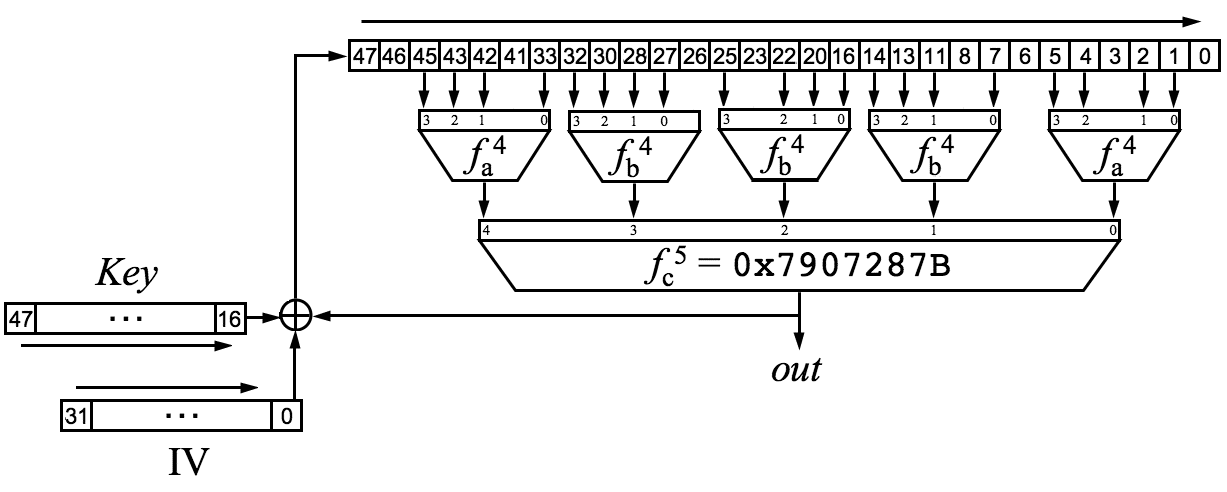
\includegraphics[width = 3in]{./figures/hitag2-2.PNG}
	\end{figure}
	
\end{frame}

\begin{frame}{Output function}

	\begin{figure}[htp]
	\centering
	\includegraphics[width = 2.5in]{./figures/output-function.PNG}
	\end{figure}
	
	\begin{figure}[htp]
	\centering
	\includegraphics[width = 3.2in]{./figures/table-mux.PNG}
	\end{figure}

\end{frame}

\begin{frame}{Keystream generation}
\begin{itemize} 
	\item Bit numbers 0, 2, 3, 6, 7, 8, 16, 22, 23, 26, 30, 41, 42, 43, 46 and 47 are used as \textit{tap} bits for updating the state
	\item Output of multiplexor $f_c^5$ constitutes the keystream bit
\end{itemize}

	\begin{figure}[htp]
	\centering
	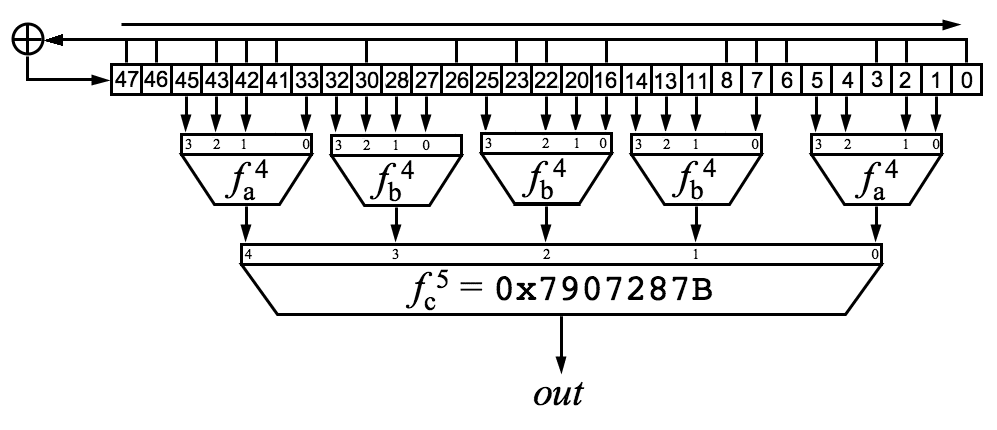
\includegraphics[width = 3in]{./figures/hitag2-3.PNG}
	\end{figure}

\end{frame}

\subsection{Motivation}
\begin{frame}{Motivation}
\begin{itemize}
	\item The internal state of HiTag2 is 48 bits
	\item A brute-force attack takes time of the order of $2^{48}$
	\item With the availability of a few hundred MB's of RAM, a time-memory tradeoff attack should be able to break HiTag2 on a PC
\end{itemize}
\end{frame}

\section{Babbage Golic time-memory tradeoff}

\subsection{Babbage Golic attack}

\begin{frame}{Basic idea of the attack}
\begin{itemize}
\small{
	\item Goal: to find one of the several occuring values of the internal state
}
\end{itemize}
	
	\begin{figure}[htp]
	\centering
	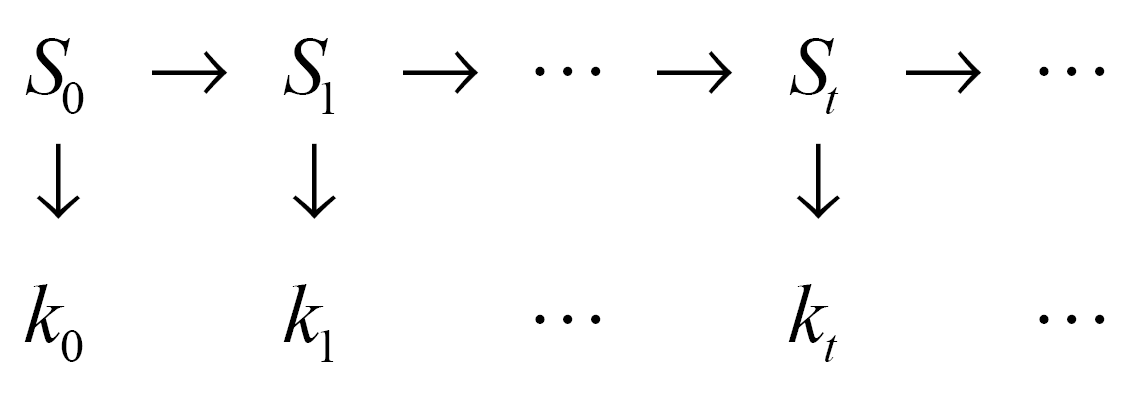
\includegraphics[width = 1.7in]{./figures/prsgmodel.PNG}
	\end{figure}

\begin{itemize}	
\small{
	\item The output sequence of certain length from a state (called \textit{prefix}) is used to uniquely identify that state
	\item Precomputation phase: $n_1$ states are randomly chosen, their prefix computed and stored
	\item Attack phase: subsequences of keystream (each corresponding to one of the $n_2$ states occuring) are matched with prefixes stored in memory
	\item According to the birthday paradox: $n_1 \times n_2 \geq 2^n$
}
\end{itemize}
\end{frame}

\begin{frame}{Parameters and tradeoff equation}

\begin{itemize}
\small{	
	\item Following parameters are used to define any tradeoff attack:
	\begin{itemize}
	\item \emph{M} represents the order of memory size required
	\item \emph{P} represents the order of time required for the precomputation phase
	\item \emph{T} represents the order of time required for the attack phase
	\item \emph{D} represents the order of prefixes available during the attack phase
	\end{itemize}
	\item \emph{M} is same as $n_1$, and \emph{T} is same as $n_2$; then we have the following tradeoff equation: $M \times T \geq 2^n$
}
\end{itemize}
\end{frame}

\begin{frame}{Attack with non-random precomputation}
\begin{itemize}
\small{
	\item Precomputation phase:
	\begin{itemize}
	\item States are not selected at random now
	\item Goal: to store states occurring at equidistant points in the huge cycle of internal states
	\item The distance between each state is then $d = 2^n/M$	
	\item An initial state $S_{initial}$ is randomly selected, and subsequenct states $S_{initial+d}$, $S_{initial+2d}$ are computed

	\end{itemize}
	\item Attack phase:
	\begin{itemize}
		\item If $d$ states occur in the keystream, then we can be sure that atleast one state would match in the memory
		\item Hence, $T$ =  $d$
	\end{itemize}
	\item Tradeoff equation:
	\begin{itemize}
		\item We can then deduce: $M \times T = 2^n$
		\item Note the difference with the tradeoff equation for random precomputation
	\end{itemize}
	
}	
\end{itemize}
\end{frame}

\begin{frame}{State transition function}
\small{
\begin{itemize}
	\item If $U$ represents the update function matrix, then the next state can be computed from curent state using the matrix multiplication: $S_{next}$ = $U . S_{current}$
	\item State transition function $A$ returns the state occurring $d$ states after a given state by:\\
	$S_{current + d}$ = $A . S_{current}$, such that $A = \underbrace{U . U . U \dots U}_{d}$
	\item An efficient way to compute matrix $A$ is: $A = \underbrace{(((U^2)^2) \dotsc )^2}_{\log_2{d}}$
	
\end{itemize}
}
\end{frame}

\section*{Summary}

\begin{frame}{Design}
\begin{itemize}
	\item Components of HiTag2:
\end{itemize}
\end{frame}

\begin{frame}{Summary}

  % Keep the summary *very short*.
  \begin{itemize}
  \item
    The \alert{first main message} of your talk in one or two lines.
  \item
    The \alert{second main message} of your talk in one or two lines.
  \item
    Perhaps a \alert{third message}, but not more than that.
  \end{itemize}
  
  % The following outlook is optional.
  \vskip0pt plus.5fill
  \begin{itemize}
  \item
    Outlook
    \begin{itemize}
    \item
      Something you haven't solved.
    \item
      Something else you haven't solved.
    \end{itemize}
  \end{itemize}
\end{frame}


\end{document}


